% Augmented Krusche comb trace: A = AB, B = ABBA (m=2, n=4).
% Same grid as fig_krusche_comb but carrying (d, delta) pairs at boundaries.
% Black-and-white only.
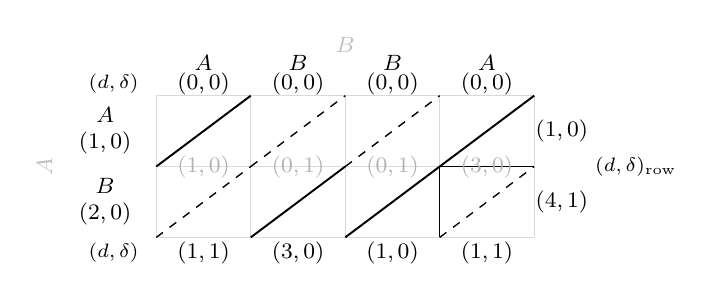
\begin{tikzpicture}[
    matchedge/.style={black, line width=0.7pt},
    missedge/.style={black, line width=0.5pt, dashed},
    swapedge/.style={black, line width=0.5pt},
    gridline/.style={gray!30, thin},
    vallabel/.style={font=\footnotesize},
    strlabel/.style={font=\footnotesize\itshape},
]

\def\cw{1.2}   % cell width (wider for (d,delta) pairs)
\def\cy{0.9}   % cell height

% ── Grid ────────────────────────────────────────────────────
\draw[gridline] (0, 0) grid[xstep=\cw, ystep=\cy] ({4*\cw}, {2*\cy});

% ── Cell diagonals ──────────────────────────────────────────
% Match cells: solid diagonal
\foreach \r/\c in {0/0, 0/3, 1/1, 1/2} {
    \pgfmathsetmacro{\px}{\c*\cw}
    \pgfmathsetmacro{\py}{(1-\r)*\cy}
    \draw[matchedge] (\px, \py) -- +({\cw}, {\cy});
}

% Mismatch cells (no swap): dashed diagonal
\foreach \r/\c in {0/1, 0/2, 1/0} {
    \pgfmathsetmacro{\px}{\c*\cw}
    \pgfmathsetmacro{\py}{(1-\r)*\cy}
    \draw[missedge] (\px, \py) -- +({\cw}, {\cy});
}

% Mismatch-swap cell (r=1, c=3): crossing
\draw[swapedge] ({3*\cw}, 0) -- +({0}, {\cy});
\draw[swapedge] ({3*\cw}, {\cy}) -- +({\cw}, {0});
\draw[missedge] ({3*\cw}, 0) -- +({\cw}, {\cy});

% ── String labels ───────────────────────────────────────────
% Reference B on top
\node[strlabel] at ({0.5*\cw}, {2*\cy + 0.42}) {$A$};
\node[strlabel] at ({1.5*\cw}, {2*\cy + 0.42}) {$B$};
\node[strlabel] at ({2.5*\cw}, {2*\cy + 0.42}) {$B$};
\node[strlabel] at ({3.5*\cw}, {2*\cy + 0.42}) {$A$};
\node[font=\footnotesize, gray!50] at ({2*\cw}, {2*\cy + 0.65}) {$B$};

% Query A on left — stacked: character above, (d_row, delta) below
\node[strlabel] at (-0.65, {1.5*\cy + 0.2}) {$A$};
\node[strlabel] at (-0.65, {0.5*\cy + 0.2}) {$B$};
\node[vallabel] at (-0.65, {1.5*\cy - 0.15}) {\footnotesize$(1,0)$};
\node[vallabel] at (-0.65, {0.5*\cy - 0.15}) {\footnotesize$(2,0)$};
\node[font=\footnotesize, gray!50, rotate=90, anchor=south]
    at (-1.2, {\cy}) {$A$};

% ── (d, delta) values at boundaries ─────────────────────────
% Top: initial (d_col, delta_col) = [(0,0), (0,0), (0,0), (0,0)]
\foreach \c in {0,...,3} {
    \node[vallabel] at ({\c*\cw + 0.5*\cw}, {2*\cy + 0.15})
        {\footnotesize$(0,0)$};
}

% Between rows: after row 0 = [(1,0), (0,1), (0,1), (3,0)]
\foreach \c/\d/\del in {0/1/0, 1/0/1, 2/0/1, 3/3/0} {
    \node[vallabel, gray!60] at ({\c*\cw + 0.5*\cw}, {\cy})
        {\footnotesize$(\d,\del)$};
}

% Bottom: final (d_col, delta_col) = [(1,1), (3,0), (1,0), (1,1)]
\foreach \c/\d/\del in {0/1/1, 1/3/0, 2/1/0, 3/1/1} {
    \node[vallabel, font=\footnotesize\bfseries]
        at ({\c*\cw + 0.5*\cw}, -0.2)
        {$(\d,\del)$};
}

% (d, delta) labels
\node[font=\scriptsize, anchor=east] at (-0.1, {2*\cy + 0.15})
    {$(d,\delta)$};
\node[font=\scriptsize, anchor=east] at (-0.1, -0.2)
    {$(d,\delta)$};

% Right: final (d_row, delta_row) = [(1,0), (4,1)]
\node[vallabel, font=\footnotesize\bfseries]
    at ({4*\cw + 0.35}, {1.5*\cy}) {$(1,0)$};
\node[vallabel, font=\footnotesize\bfseries]
    at ({4*\cw + 0.35}, {0.5*\cy}) {$(4,1)$};

% d_row label
\node[font=\scriptsize, anchor=west] at ({4*\cw + 0.65}, {\cy})
    {$(d,\delta)_{\mathrm{row}}$};

\end{tikzpicture}
